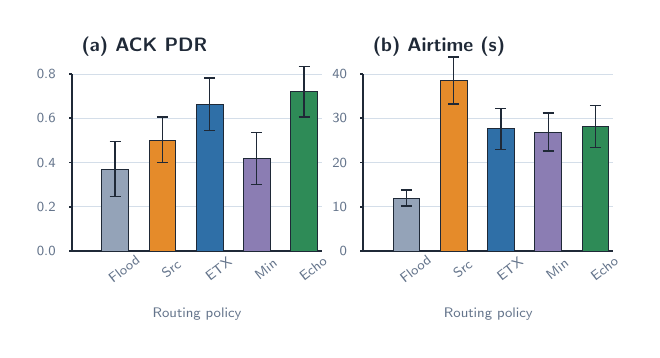
\begin{tikzpicture}[
    font=\sffamily\tiny,
    axis/.style={draw=ink, line width=0.55pt},
    gridline/.style={draw=grid, line width=0.3pt},
    tick/.style={font=\sffamily\tiny, text=muted},
    value/.style={font=\sffamily\tiny, text=ink, anchor=south},
    whisker/.style={draw=ink, line width=0.45pt},
    bar/.style={draw=ink, line width=0.25pt}
]
\definecolor{ink}{HTML}{1F2937}
\definecolor{muted}{HTML}{64748B}
\definecolor{grid}{HTML}{D4DEE9}
\definecolor{flood}{HTML}{94A3B8}
\definecolor{source}{HTML}{E58B2A}
\definecolor{metric}{HTML}{2F6FA7}
\definecolor{minhop}{HTML}{8B7DB3}
\definecolor{meshecho}{HTML}{2E8B57}

\def\H{2.25}
\def\W{3.18}
\def\gap{0.52}
\def\panelshift{3.70}
\def\barw{0.34}
\def\xone{0.38}
\def\xtwo{0.98}
\def\xthree{1.58}
\def\xfour{2.18}
\def\xfive{2.78}

% (a) ACK-confirmed PDR, y range 0--0.8.
\begin{scope}
  \foreach \y/\lab in {0/0.0,0.5625/0.2,1.125/0.4,1.6875/0.6,2.25/0.8} {
    \draw[gridline] (0,\y) -- (\W,\y);
    \draw[axis] (0,\y) -- ++(-0.035,0);
    \node[tick, anchor=east] at (-0.08,\y) {\lab};
  }
  \draw[axis] (0,0) -- (0,\H);
  \draw[axis] (0,0) -- (\W,0);
  \node[font=\sffamily\scriptsize\bfseries, text=ink, anchor=south west]
    at (0,\H+0.10) {(a) ACK PDR};

  % Means: .371, .502, .661, .419, .720. 95% CI half-widths:
  % .124, .103, .119, .118, .115.
  \fill[bar, fill=flood] (\xone,0) rectangle ++(\barw,1.0434);
  \fill[bar, fill=source] (\xtwo,0) rectangle ++(\barw,1.4124);
  \fill[bar, fill=metric] (\xthree,0) rectangle ++(\barw,1.8628);
  \fill[bar, fill=minhop] (\xfour,0) rectangle ++(\barw,1.1784);
  \fill[bar, fill=meshecho] (\xfive,0) rectangle ++(\barw,2.0250);

  \foreach \x/\m/\lo/\hi in {
      \xone/1.0434/0.6941/1.3928,
      \xtwo/1.4124/1.1222/1.7027,
      \xthree/1.8628/1.5280/2.1981,
      \xfour/1.1784/0.8468/1.5100,
      \xfive/2.0250/1.7016/2.3484} {
    \draw[whisker] (\x+0.17,\lo) -- (\x+0.17,\hi);
    \draw[whisker] (\x+0.10,\lo) -- (\x+0.24,\lo);
    \draw[whisker] (\x+0.10,\hi) -- (\x+0.24,\hi);
  }

  \foreach \x/\lab in {
      \xone/Flood,
      \xtwo/Src,
      \xthree/ETX,
      \xfour/Min,
      \xfive/Echo} {
    \node[tick, anchor=north, rotate=38] at (\x+0.17,-0.08) {\lab};
  }
  \node[tick, anchor=north] at (\W/2,-0.60) {Routing policy};
\end{scope}

% (b) Total airtime, y range 0--40 s.
\begin{scope}[xshift=\panelshift cm]
  \foreach \y/\lab in {0/0,0.5625/10,1.125/20,1.6875/30,2.25/40} {
    \draw[gridline] (0,\y) -- (\W,\y);
    \draw[axis] (0,\y) -- ++(-0.035,0);
    \node[tick, anchor=east] at (-0.08,\y) {\lab};
  }
  \draw[axis] (0,0) -- (0,\H);
  \draw[axis] (0,0) -- (\W,0);
  \node[font=\sffamily\scriptsize\bfseries, text=ink, anchor=south west]
    at (0,\H+0.10) {(b) Airtime (s)};

  % Means: 12.0, 38.5, 27.6, 26.9, 28.1. 95% CI half-widths:
  % 1.8, 5.3, 4.6, 4.3, 4.7.
  \fill[bar, fill=flood] (\xone,0) rectangle ++(\barw,0.6750);
  \fill[bar, fill=source] (\xtwo,0) rectangle ++(\barw,2.1656);
  \fill[bar, fill=metric] (\xthree,0) rectangle ++(\barw,1.5525);
  \fill[bar, fill=minhop] (\xfour,0) rectangle ++(\barw,1.5131);
  \fill[bar, fill=meshecho] (\xfive,0) rectangle ++(\barw,1.5806);

  \foreach \x/\m/\lo/\hi in {
      \xone/0.6750/0.5738/0.7763,
      \xtwo/2.1656/1.8671/2.4641,
      \xthree/1.5525/1.2938/1.8113,
      \xfour/1.5131/1.2713/1.7549,
      \xfive/1.5806/1.3163/1.8449} {
    \draw[whisker] (\x+0.17,\lo) -- (\x+0.17,\hi);
    \draw[whisker] (\x+0.10,\lo) -- (\x+0.24,\lo);
    \draw[whisker] (\x+0.10,\hi) -- (\x+0.24,\hi);
  }

  \foreach \x/\lab in {
      \xone/Flood,
      \xtwo/Src,
      \xthree/ETX,
      \xfour/Min,
      \xfive/Echo} {
    \node[tick, anchor=north, rotate=38] at (\x+0.17,-0.08) {\lab};
  }
  \node[tick, anchor=north] at (\W/2,-0.60) {Routing policy};
\end{scope}
\end{tikzpicture}
